\documentclass[conference]{IEEEtran}
\IEEEoverridecommandlockouts

\usepackage{cite}
\usepackage{subcaption}
\usepackage{amsmath,amssymb,amsfonts}
\usepackage{graphicx}
\usepackage{xcolor}
\usepackage{hyperref}
\usepackage{booktabs} % For better table lines
% Better spacing
\setlength{\textfloatsep}{8pt}
\setlength{\intextsep}{8pt}
\setlength{\floatsep}{8pt}
\vspace{-5pt}


\begin{document}

\title{2D Advection-Diffusion Benchmark: Serial, OpenMP, and CUDA Implementations}

\author{
\IEEEauthorblockN{Siddhant Tyagi}
\IEEEauthorblockA{B22278\\
Department of Electrical Engineering\\
IIT Mandi, India
}
\and
\IEEEauthorblockN{Adithya Raju Nair}
\IEEEauthorblockA{B22186\\
Department of Electrical Engineering\\
IIT Mandi, India
}
}

\maketitle

\begin{abstract}
This work presents the development and performance benchmarking of a 2D Advection-Diffusion solver, a fundamental component in atmospheric and fluid dynamics simulations. Three implementations are developed: a baseline serial version, a shared-memory parallel version using OpenMP for multi-core CPUs, and a GPU-accelerated version using CUDA. The solver employs finite difference approximations and explicit time-stepping on a discretized grid, initialized with a central heat pulse. Performance is evaluated across varying grid sizes, focusing on execution time per step and speedup ratios. The CUDA implementation is designed with memory coalescing in mind to maximize GPU efficiency. Results highlight the significant performance gains achieved through parallelization, particularly with CUDA, demonstrating the scalability and efficiency of GPU computing for stencil-based computations.
\end{abstract}

\begin{IEEEkeywords}
Advection-Diffusion, CUDA, OpenMP, HPC, Parallel Computing, Finite Difference, GPU, CPU
\end{IEEEkeywords}

\section{Introduction}

The simulation of atmospheric and fluid dynamics phenomena, such as heat transfer, pollutant dispersion, and weather forecasting, often relies on solving partial differential equations that describe advection and diffusion processes. The 2D Advection-Diffusion equation serves as a fundamental model for understanding the transport of scalar quantities within a fluid flow.

The computational intensity of these simulations, especially for large grid sizes and long simulation times, necessitates the use of parallel computing techniques. This project focuses on developing a simplified 2D Advection-Diffusion solver and benchmarking its performance across different parallelization paradigms: a baseline serial implementation, a multi-core CPU parallelization using OpenMP, and a GPU-accelerated version leveraging CUDA.

The primary objective is to evaluate the performance gains, speedup, and scalability achieved by these parallel implementations compared to the serial counterpart. The solver utilizes finite difference approximations for spatial derivatives and explicit time-stepping for temporal evolution on a discretized grid, initialized with a central heat pulse. Special attention is given to optimizing the CUDA kernel for memory coalescing to maximize GPU efficiency.

\subsection{AI Usage Statement}

This work involved the use of AI-assisted tools to support code structuring, debugging, and formatting of the final report. The core implementation, analysis, and interpretation of results were carried out independently, with AI tools serving as an aid for improving clarity and efficiency in development and documentation.

\section{Mathematical Formulation}

The 2D Advection-Diffusion equation describes the change in concentration \(U\) of a scalar quantity over time due to both diffusion and advection (convection) processes. It can be written as:

\begin{equation}
\frac{\partial U}{\partial t} = D \left( \frac{\partial^2 U}{\partial x^2} + \frac{\partial^2 U}{\partial y^2} \right) - \left( V_x \frac{\partial U}{\partial x} + V_y \frac{\partial U}{\partial y} \right)
\end{equation}

where \(U(x, y, t)\) is the scalar quantity, \(D\) is the diffusion coefficient, \(V_x\) and \(V_y\) are the advection velocities in the x and y directions, respectively.

For numerical solution, we employ finite difference approximations for spatial derivatives and an explicit forward Euler scheme for time integration. The discretized equation for a grid point \((i, j)\) at time \(t\) becomes:

{\small
\begin{align*}
U_{i,j}^{t+1} = U_{i,j}^t &+ \Delta t \left[ D \left( \frac{U_{i+1,j}^t - 2U_{i,j}^t + U_{i-1,j}^t}{(\Delta x)^2} + \frac{U_{i,j+1}^t - 2U_{i,j}^t + U_{i,j-1}^t}{(\Delta y)^2} \right) \right. \\
&\left. - \left( V_x \frac{U_{i+1,j}^t - U_{i-1,j}^t}{2\Delta x} + V_y \frac{U_{i,j+1}^t - U_{i,j-1}^t}{2\Delta y} \right) \right]
\end{align*}
}

where \(\Delta t\) is the time step, \(\Delta x\) and \(\Delta y\) are the grid spacings. Fixed boundary conditions are applied, meaning the values at the grid edges remain constant throughout the simulation.

\section{Implementation and Profiling}

The 2D Advection-Diffusion solver was implemented in C++ with three distinct execution modes: Serial, OpenMP, and CUDA.

\subsection{Heat Pulse Initialization}
The simulation grid is initialized with a "Heat Pulse" in the center. This involves setting a circular region in the middle of the grid to a high value, which then diffuses and advects across the domain. This provides a clear initial condition to observe the transport phenomena.

\subsection{Serial Implementation}
The baseline serial implementation uses standard C++ nested loops to iterate over the grid points and apply the finite difference update rule. This serves as the reference for performance comparison.

\subsection{OpenMP Implementation}
For multi-core CPU parallelization, OpenMP pragmas were utilized. The main time-stepping loop, which involves iterating over the grid points to compute the new state, was parallelized using \#pragma omp parallel for collapse(2)\. This distributes the workload across available CPU cores, aiming to reduce execution time.

\subsection{CUDA Implementation}
The GPU-accelerated implementation leverages NVIDIA's CUDA platform. The core computation of updating each grid point is offloaded to a CUDA kernel (\texttt{advectionDiffusionKernel}).
\begin{itemize}
    \item \textbf{Kernel Structure:} Each thread in the CUDA grid is responsible for computing the update for a single grid point \((i, j)\).
    \item \textbf{Memory Management:} Data is transferred from host (CPU) memory to device (GPU) memory before computation and results can be transferred back if needed. Double buffering is used on the device to swap \texttt{U\_old} and \texttt{U\_new} pointers efficiently.
    \item \textbf{Memory Coalescing:} To maximize GPU memory bandwidth, threads are mapped such that adjacent threads within a warp access contiguous memory locations. Specifically, the column index \texttt{j} is mapped to \texttt{threadIdx.x}, promoting coalesced global memory reads and writes for the \texttt{U\_old[idx]} and \texttt{U\_new[idx]} accesses. While accesses in the \texttt{y} direction (\texttt{U\_old[idx + N]}, \texttt{U\_old[idx - N]}) are not perfectly coalesced, the \texttt{x} direction coalescing provides significant performance benefits.
\end{itemize}

\subsection{Performance Metrics}
Performance was evaluated by measuring the average time taken per simulation step for each implementation across various grid sizes. The speedup \(S(p)\) is calculated as the ratio of the serial execution time to the parallel execution time for a given grid size:

\begin{equation}
S(p) = \frac{T_{\text{Serial}}}{T_{\text{Parallel}}}
\end{equation}

where \(T_{\text{Serial}}\) is the time per step for the serial implementation, and \(T_{\text{Parallel}}\) is the time per step for the OpenMP or CUDA implementation.

\begin{table}[!t]
\centering
\caption{Performance Results: Time Per Step (seconds)}
\label{tab:performance}
\begin{tabular}{cccc}
\toprule
\textbf{Size} & \textbf{Serial} & \textbf{OpenMP} & \textbf{CUDA} \\
\midrule
64 & 0.0000620755 & 0.0000653830 & 0.0000256594 \\
128 & 0.0002702835 & 0.0004018155 & 0.0000252189 \\
256 & 0.0012300442 & 0.0009842358 & 0.0000923751 \\
512 & 0.0064070777 & 0.0087243109 & 0.0004006349 \\
1024 & 0.0371885943 & 0.0220560860 & 0.0015107485 \\
\bottomrule
\end{tabular}
\end{table}

\begin{table}[!t]
\centering
\caption{Speedup Ratios (vs. Serial)}
\label{tab:speedup}
\begin{tabular}{ccc}
\toprule
\textbf{Size} & \textbf{OpenMP Speedup} & \textbf{CUDA Speedup} \\
\midrule
64 & 0.95 & 2.42 \\
128 & 0.67 & 10.72 \\
256 & 1.25 & 13.31 \\
512 & 0.73 & 16.00 \\
1024 & 1.69 & 24.62 \\
\bottomrule
\end{tabular}
\end{table}

\section{Results and Discussion}

The performance results, summarized in Table~\ref{tab:performance} and Table~\ref{tab:speedup}, demonstrate the varying efficiencies of the different implementations across increasing grid sizes.

\begin{figure}[!t]
\centering
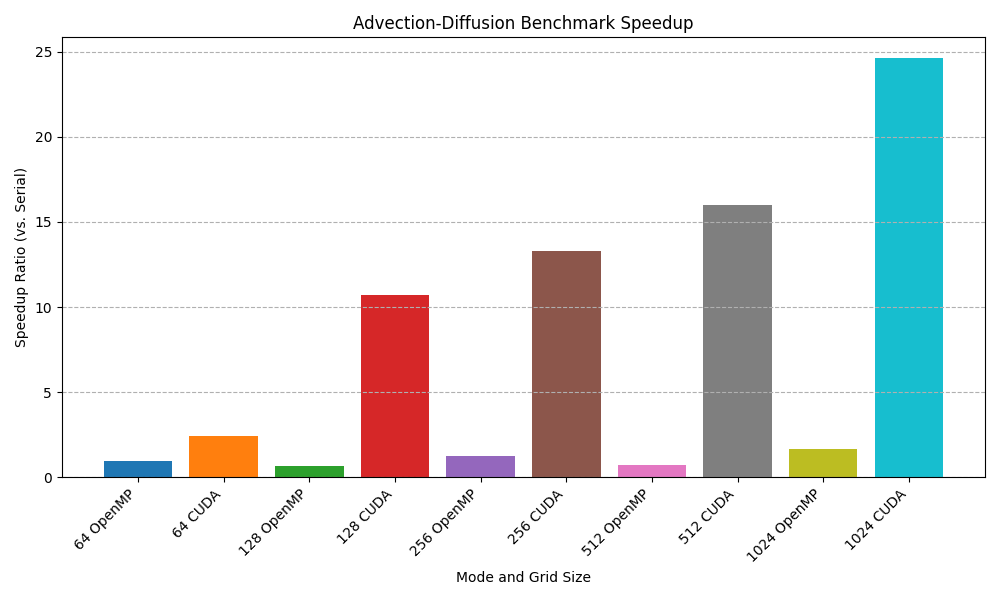
\includegraphics[width=0.8\columnwidth]{speedup_plot.png}
\caption{Speedup ratios of OpenMP and CUDA implementations relative to the Serial implementation across different grid sizes.}
\label{fig:speedup_plot}
\end{figure}

For smaller grid sizes (e.g., 64x64), the overheads associated with parallelization (thread creation, synchronization, data transfer) can sometimes outweigh the benefits, as seen with OpenMP showing a slight slowdown for 64x64 and 128x128 grids. However, as the grid size increases, the computational workload grows, and the advantages of parallelization become evident.

The OpenMP implementation shows modest speedups for larger grid sizes (e.g., 1.69x for 1024x1024), indicating effective utilization of multi-core CPUs. The speedup is not linear, which is typical for shared-memory parallelization due to factors like memory bandwidth contention, cache effects, and synchronization overheads.

The CUDA implementation consistently delivers the most significant performance improvements. For the largest grid size (1024x1024), CUDA achieves a speedup of approximately 24.62x over the serial version. This substantial gain highlights the power of GPU parallelism for highly parallelizable, stencil-based computations. The focus on memory coalescing in the CUDA kernel contributes to this efficiency by optimizing global memory access patterns.

The speedup trends indicate that as the problem size increases, the relative performance advantage of the parallel implementations, especially CUDA, becomes more pronounced, demonstrating good scalability for larger simulations.

\section{Flow Visualization and Mountain Pass Simulation}

\subsection{Visualization of Temperature and Velocity Fields}

To better understand the physical behavior of the system, the temperature field was visualized as a heatmap and overlaid with velocity vectors using quiver plots. The heatmap represents the scalar field \(U(x,y,t)\), while the arrows indicate the local velocity components \((V_x, V_y)\).

These visualizations allow simultaneous observation of:
\begin{itemize}
    \item Advection: transport of heat along the flow direction
    \item Diffusion: spreading and smoothing of the heat distribution
    \item Flow structure: direction and magnitude of the wind field
\end{itemize}

Snapshots were recorded at regular time intervals to capture the temporal evolution of the system.

\begin{figure}[!t]
\centering

\begin{subfigure}[b]{\columnwidth}
    \centering
    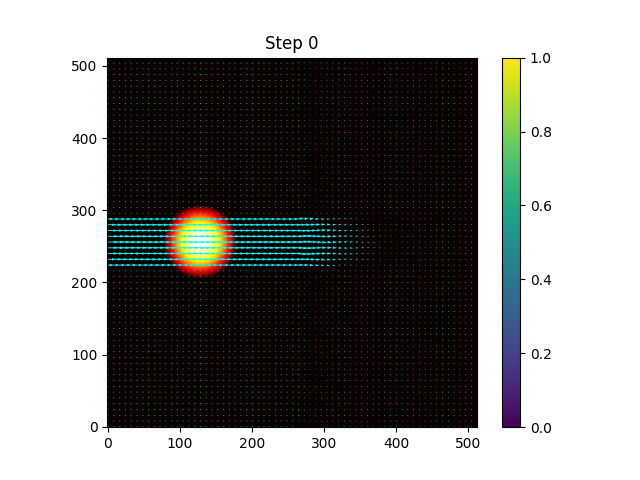
\includegraphics[width=\linewidth]{step0.png}
    \caption{Step 0}
\end{subfigure}
\hfill
\begin{subfigure}[b]{\columnwidth}
    \centering
    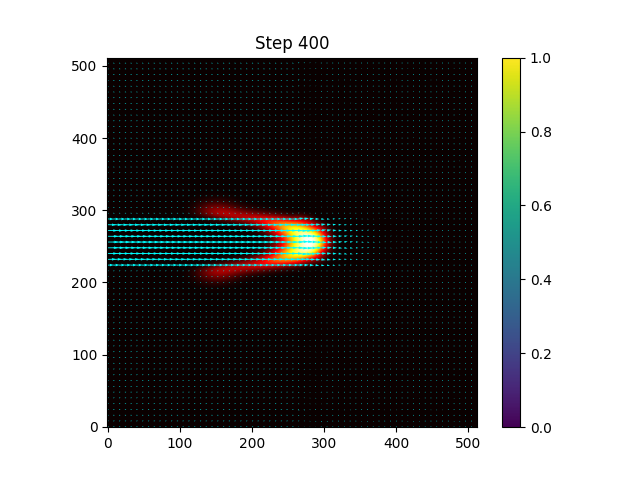
\includegraphics[width=\linewidth]{step400.png}
    \caption{Step 400}
\end{subfigure}
\hfill
\begin{subfigure}[b]{\columnwidth}
    \centering
    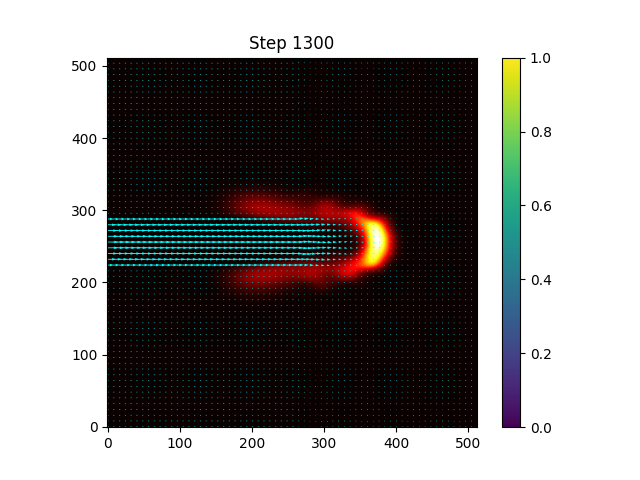
\includegraphics[width=\linewidth]{step1300.png}
    \caption{Step 1300}
\end{subfigure}

\caption{Evolution of the heat pulse as it advects through the mountain pass. The pulse accelerates within the constriction and spreads downstream due to velocity decay and diffusion.}
\label{fig:three_steps}
\end{figure}

\subsection{Mountain Pass Velocity Field}

To simulate realistic atmospheric flow, a spatially varying velocity field was designed to model wind passing through a narrow mountain pass. The domain consists of a central low-resistance region (the pass) and high-resistance regions (mountains) on either side.

The velocity field is constructed using:
\begin{itemize}
    \item A Gaussian profile centered along the pass to create a high-speed jet
    \item A smooth sigmoid transition to represent the boundary between the pass and the mountains
    \item A vertical velocity component to model flow deflection and bending
\end{itemize}

Within the narrow pass, the horizontal velocity \(V_x\) increases significantly due to constriction, while outside the pass it remains small. Downstream of the pass, the flow is modified to include:
\begin{itemize}
    \item Velocity decay to simulate loss of momentum
    \item Lateral expansion using a transverse velocity component \(V_y\)
    \item Mild turbulence to induce mixing
\end{itemize}

This produces a jet-like structure that accelerates within the pass and spreads outward after exiting it.

\subsection{Advection of Heat Pulse Through the Pass}

The simulation is initialized with a localized heat pulse placed upstream of the mountain pass. As time progresses, this pulse is transported by the velocity field.

Inside the pass, the heat pulse accelerates due to the increased velocity, resulting in a narrow, elongated structure. After exiting the pass, the combined effects of velocity decay, lateral expansion, and diffusion cause the pulse to spread outward, forming a fan-like pattern.

The observed behavior highlights the interaction between:
\begin{itemize}
    \item Advection, which transports the heat along streamlines
    \item Diffusion, which smooths and spreads the temperature field
\end{itemize}

This setup provides a simplified but effective model of transport phenomena such as wind flow through terrain and pollutant dispersion in atmospheric systems.

\section{Conclusion}

A 2D Advection-Diffusion solver was successfully implemented and benchmarked using Serial, OpenMP, and CUDA approaches. The project demonstrated the application of finite difference methods and explicit time-stepping for simulating transport phenomena.

Profiling revealed that parallelization significantly reduces execution time, with CUDA providing the most substantial speedup, achieving up to 24.62x for a 1024x1024 grid. OpenMP also offered performance improvements for larger grid sizes, albeit more modestly. The results underscore the effectiveness of GPU computing for computationally intensive, grid-based simulations and the importance of memory access optimization techniques like coalescing in CUDA.

Future work could involve implementing more advanced numerical schemes (e.g., implicit methods), exploring different boundary conditions, and integrating more complex physical phenomena to build a more comprehensive weather simulation framework.
\balance
\end{document}
